\documentclass[a4paper,12pt]{article}
\usepackage[ngerman]{babel}
\usepackage{multirow}
\usepackage{xltxtra}
\usepackage[utf8x]{inputenc}
\usepackage{fontspec}
\usepackage{eurosym}
\usepackage{amsfonts}
\usepackage{graphicx}
\usepackage[paper=a4paper,left=25mm,right=25mm,top=25mm,bottom=25mm]{geometry}
\usepackage{makecell}
\usepackage[table]{xcolor}
\usepackage{float}
\usepackage[normalem]{ulem}
\usepackage{xcolor,colortbl}
\definecolor{Gray}{gray}{0.85}
\usepackage[automark]{scrlayer-scrpage}
\usepackage[
	colorlinks=true,
	urlcolor=blue,
	linkcolor=green
]{hyperref}
\setlength{\parindent}{0em}
\setlength{\parskip}{1ex}
\pagestyle{scrheadings}
\clearscrheadfoot
\usepackage[defaultsans]{droidsans}
\renewcommand*\familydefault{\sfdefault}
\begin{document}
\input{theme.tex}
\input{version.tex}
\newcommand{\combineDivisions}{Hinweis: Wenn weniger als 5 Teams in einer der
Altersgruppen angemeldet sind, hat die Veranstaltungsleitung die Möglichkeit,
Altersgruppen zusammenzulegen. }

\newcommand{\declareExhibition}{Wenn insgesamt weniger als 5 Teams angemeldet
sind kann die Veranstaltung zur Ausstellung erklärt werden. }

\newcommand{\robotRequirements}{Autonomer Roboter, basierend auf einer
beliebigen Plattform, der \euro{1.500} oder weniger kostet und die folgenden
Designbedingungen erfüllt, die beim Check-In überprüft werden:}


\newcommand{\tournamentScoring}{
\begin{figure}[H]
	\centering
	\def\svgwidth{\columnwidth}
	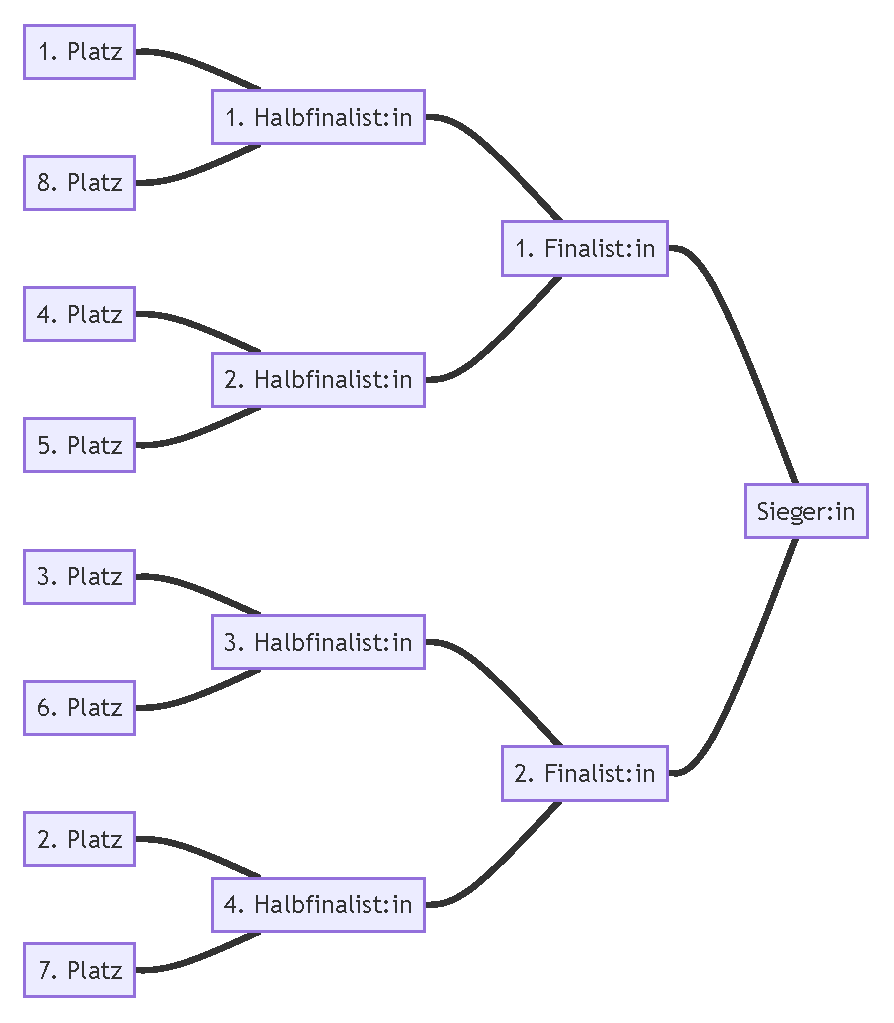
\includegraphics{tournament_score/tournament_score.pdf}
\end{figure}
}

\newcommand{\tournamentQualification}{Die aufsteigenden Teams werden
entsprechend ihrer Gesamtpunktzahl in den Turnierplan eingetragen (unten findet
ihr ein Beispiel für ein typisches Turnier mit 8 Teams). }

\newcommand{\combinedTournament}{
Hinweis: Wenn weniger als 8 Teams in allen Altersgruppen angemeldet sind, hat
die Veranstaltungsleitung die Möglichkeit, den Turnierplan entsprechend
anzupassen.
}

\newcommand{\scoreRuns}{
Die besten (8) Teams, welche am Turnier teilnehmen, werden wie folgt ermittelt:
\begin{itemize}
	\item Die Veranstaltungsleitung legt fest wieviele Läufe pro Team
		offiziell gewertet werden dürfen.
	\item Davon gehen die besten Wertungen in die Gesamtpunktzahl ein.
	\item Die Veranstaltungsleitung legt fest wieviele der offiziell
		gewerteten Läufen in die Gesamtpunktzahl eingehen.
	\item Auf Grundlage dieser Gesamtpunktzahl werden die besten Teams
		ermittelt, welche am Turnier teilnehmen.
\end{itemize}
}

\newcommand{\lightConditions}{
Die Challenge kann in Bereichen mit natürlichen Licht stattfinden, welches die
Lichtverhältnisse auf dem Spielplan verändern kann. Teams sollten darauf
vorbereitet sein, diese natürlichen Bedingungen zu meistern. }

\ohead{Regelstand: \commitDate, id: \commitID}
\title{\tagYear\ Entrepreneurial Challenge Regeln}

\makeatletter
\let\inserttitle\@title
\makeatother
\begin{center}
	\rrgerLogo
	\huge                      % Schriftgröße einstellen
	\bfseries                   % Fettdruck einschalten
	\\
	\inserttitle
\end{center}

\section{Ziel}
Vermarkte mit den Stimmen aller Besucher der Veranstaltung ein innovatives und
funktionales (autonomes und/oder ferngesteuertes) Roboterprodukt, das Kunden
haben möchten.

\section{Wer kann teilnehmen?}
Teams aus 2 bis 4 Spieler:innen in \textbf{getrennten Altersgruppen}:

\begin{itemize}
	\item Grundschule (ES) und Mittelstufe (MS)
	\item Oberstufe (HS) und Universität/Beruf (UP)
\end{itemize}
\combineDivisions
\declareExhibition

\section{Anforderungen}
Autonomes oder ferngesteuertes funktionierendes Robotik-Produkt, basierend auf
beliebiger Plattform, das \euro{3.000} oder weniger kostet und die folgenden
Designbedingungen erfüllt, die beim Check-In überprüft werden:
\begin{enumerate}
	\item Demonstration der Funktionsweise des Produkts (weist eine
		Eingabe-Verarbeitung-Ausgabe-Logik auf).
	\item Vorlage von Team-Visitenkarten mit Logo.
	\item Vorlage eines 1-seitigen Marketing-Flyers bereit zur
		Veröffentlichung.
	\item Vorlage der Materialien für eure Ausstellungsfläche.
	\begin{enumerate}
		\item Bei Präsenzveranstaltungen werden euch 2 Stühle, Strom
			und öffentliches Internet zur Verfügung gestellt.
			Alle anderen Materialien werden von eurem Team selbst
			gestellt.
	\end{enumerate}
	\item In der HS/UP-Altersgruppe müssen die Teams ein hochwertiges,
		60-90 Sekunden langes Werbevideo vorlegen.
\end{enumerate}

\section{Allgemeine Spielregeln}
\begin{enumerate}
	\item  Robotik-System: definiert als jedes Produkt, das eine
		EINGABE-VERARBEITUNGS-AUSGABE-Logik enthält. (z.B. fallen unter
		die Definition: Apps, Mobiltelefon, Fernseher mit
		TV-Fernbedienung, Auto mit Transponderschlüssel, Laptop, ...)
	\item Vermarktung eines funktionierenden Robotik-Systems an ALLE
		VERANSTALTUNGSBESUCHER als "`Kunden"'.
	\item Alle Teilnehmer haben eine einzige Stimme, die sie für ein
		Entrepreneurial Produkt abgeben können.
	\item AUSNAHME: Eine Jury aus Fachexperten ("`Subject Matter Experts"',
		SME) haben 50 Stimmen, die sie für ein oder mehrere Produkte
		abgeben können.
\end{enumerate}

\section{Challenge Spezifikation}
\begin{enumerate}
\item Zur Verfügung stehen:
	\begin{enumerate}
		\item $3 m \times 3 m$ Standfläche; auf Wunsch auch größer
		\item Stromversorgung
		\item Öffentliches Internet
		\item Stühle (2)
		\item KEIN TISCH. Für die Einrichtung des Standes seid ihr zu
			100 \% selbst verantwortlich.
	\end{enumerate}
	\item Richtlinien für das Verkaufsteam:
	\begin{enumerate}
		\item Muß aus EUREN ANGEMELDETEN Teammitgliedern bestehen.
		\item Wenn nicht registrierte Personen helfen, wird eine Strafe
			von 100 Stimmen pro nicht registrierter Person auf die
			Gesamtpunktzahl des Teams erhoben.
		\item Es steht euch frei (und ihr seid dazu ermutigt), euch
			auf der Veranstaltung zu bewegen, um Kunden an euren
			Stand zu locken.
	\end{enumerate}
	\item Abstimmung
        \begin{enumerate}
		\item Präsenzveranstaltung: s. Zeitplan der Veranstaltung
		\item Alle Stimmen werden über ein auf der Veranstaltung
			ausgewiesenes Wahlsystem abgegeben.
        \end{enumerate}
	\item ALLE Besucher der Veranstaltung können abstimmen (d.h. alle
		vor Ort befindlichen Teams, Familien, Zuschauer und Mitarbeiter
		der Veranstaltung sind stimmberechtigt).
\end{enumerate}

\section{Punktevergabe}
\renewcommand{\labelitemi}{$\star$}
\renewcommand{\labelitemii}{$\checkmark$}
\begin{itemize}
	\item Eine (1) Stimme wird jedem Besucher der Veranstaltung während des
		Abstimmungszeitraums gewährt.
	\item Fachexperten (SME) haben fünfzig (50) Stimmen, die sie für jedes
		Projekt verwenden können. Sie können alle oder einen Teil ihrer
		50 Stimmen für ein Projekt abgeben, wiederum während des
		Abstimmungszeitraums.
	\item Die Projekte mit den höchsten Stimmzahlen werden in den
		ausgeschriebenen Kategorien (die von der jeweiligen
		Veranstaltungsleitung festgelegt werden) mit Preisen bedacht.
	\item Mögliche Kategorien sind u.a. folgende Themen, aber nicht nur:
	\begin{itemize}
		\item Präsentationen (dein Vortrag)
		\item Video, Werbefilm (HS/UP-Altersgruppe)
		\item Beste Besucherwertung
		\item Beste SME-Wertung
		\item Einzigartiges Konzept
		\item Einblick in euer Produkt (euer Code)
	\end{itemize}
\end{itemize}
\end{document}
